% Chapter 4

\chapter{CA Guide Mobile Application} % Main chapter title

\label{frontend} % For referencing the chapter elsewhere, use \ref{Chapter1} 

\lhead{Chapter 4. \emph{CA Guide Frontend}} % This is for the header on each page - perhaps a shortened title

%----------------------------------------------------------------------------------------

\section{Introduction and Goal}

The CA Guide mobile application has to display predefined textual descriptions of sites areas, show images and play audio files when a specific context state is reached. The trigger will often be entering a specified area at a moderate pace that signals the visitor is interested and not only passing by to reach another place. But also leaving an area can be of interest, for example to indicate single subareas that were missed. Even offering a coffee break discount coupon on the display after the visitor made 5000 steps through the park or exhibition is imaginable.

An essential aspect is the ability to record and replay the data coming from all accessed sensors. That's the only way to effectively develop a context-sensitive application and so special attention has to be given to this part of the system.

\section{The Target Platform}

The target mobile platform for the CA Guide front end application is iOS 8.1. The targeted mobile device is an iPad mini 2 with GPS sensor. This device was chosen for it's compact size and light weight, while still offering much more screen size than a normal smartphone, which is advantageous for displaying images and text in a size that is more comfortable to read.

\section{Setting Up the Development Platform}

This mobile application is written in Swift 1.2 using the native Apple XCode IDE in version 6.3, which at the time of writing is still in beta status\footnote{In fact, the last "stable" version 6.1, which I used for several weeks before, crashed too quite often with the Message so I decided to use the newest beta IDE version, that proved not to be more buggy than the release version while offering the newest Swift Compiler with several optimizations in compile and runtime performance.}. It can be downloaded at \cite{xcodebeta}.


For logging purposes, CocoaLumberjack \cite{cocoalumberjack}
was used. In contrast to the logging system shipped with the iOS SDK, it offers several logging levels and has a much greater performance \cite{clperf}. 
This is especially important when logging low level functions like the one handling accelerometer updates every 10ms.

To add extensions like CocoaLumberjack to the project, the dependency management system CocoaPods \cite{cocoapods}
was used. It creates a XCode Workspace containing the own project paired with a managed CocoaPods project containing all the extra libraries. The wanted libraries are specified in a file named "Podfile", where you define the ids and the desired version for each build target. 

\begin{lstlisting}[caption={The CocoaPods file of the CA Guide front end XCode project},basicstyle=\small\ttfamily,language=c,aboveskip=15pt]
target 'Guide' do
   pod 'CocoaLumberjack', '2.0.0-beta'
   pod 'couchbase-lite-ios', '~> 1.0'
   pod 'CorePlot', :git => 'https://github.com/core-plot/core-plot.git', :branch => 'release-2.0'
end

target 'GuideTests' do
   pod 'CocoaLumberjack', '2.0.0-beta'
   pod 'couchbase-lite-ios', '~> 1.0'
end
\end{lstlisting}


Libraries not available in the public CocoaPods repository can be added defining a custom git url and branch, as was done for Core Plot \cite{coreplot}, an open source plotting framework used for plotting beacon signal strength on debug screens. 

Because at the time of writing many modules are written in Objective-C, a so-called bridging header file
has to be added manually to the own Swift project to expose the Ojective-C headers to the Swift compiler and let it automatically create a Swift API that can be used in the own Swift code \cite[p. 71, chapter "Importing Objective-C into Swift"]{swift-objc-book}.

\section{Architecture}

Below the presentation layer and the application logic, a clean sensor data processing foundation that provides the context information for the application has to be designed. This foundation is divided in three logical layers. At the bottom are the sensor data sources, consisting of the iOS sensor APIs and virtual sensors. As processing of sensor data is best done in several steps, as we will see in this chapter, two layers of sensor data processing are added, the first for low-level  algorithms called at higher frequency and the second for higher level ones, performing more computation-intensive tasks at a lower frequency.  

\begin{figure}[H]
\centering
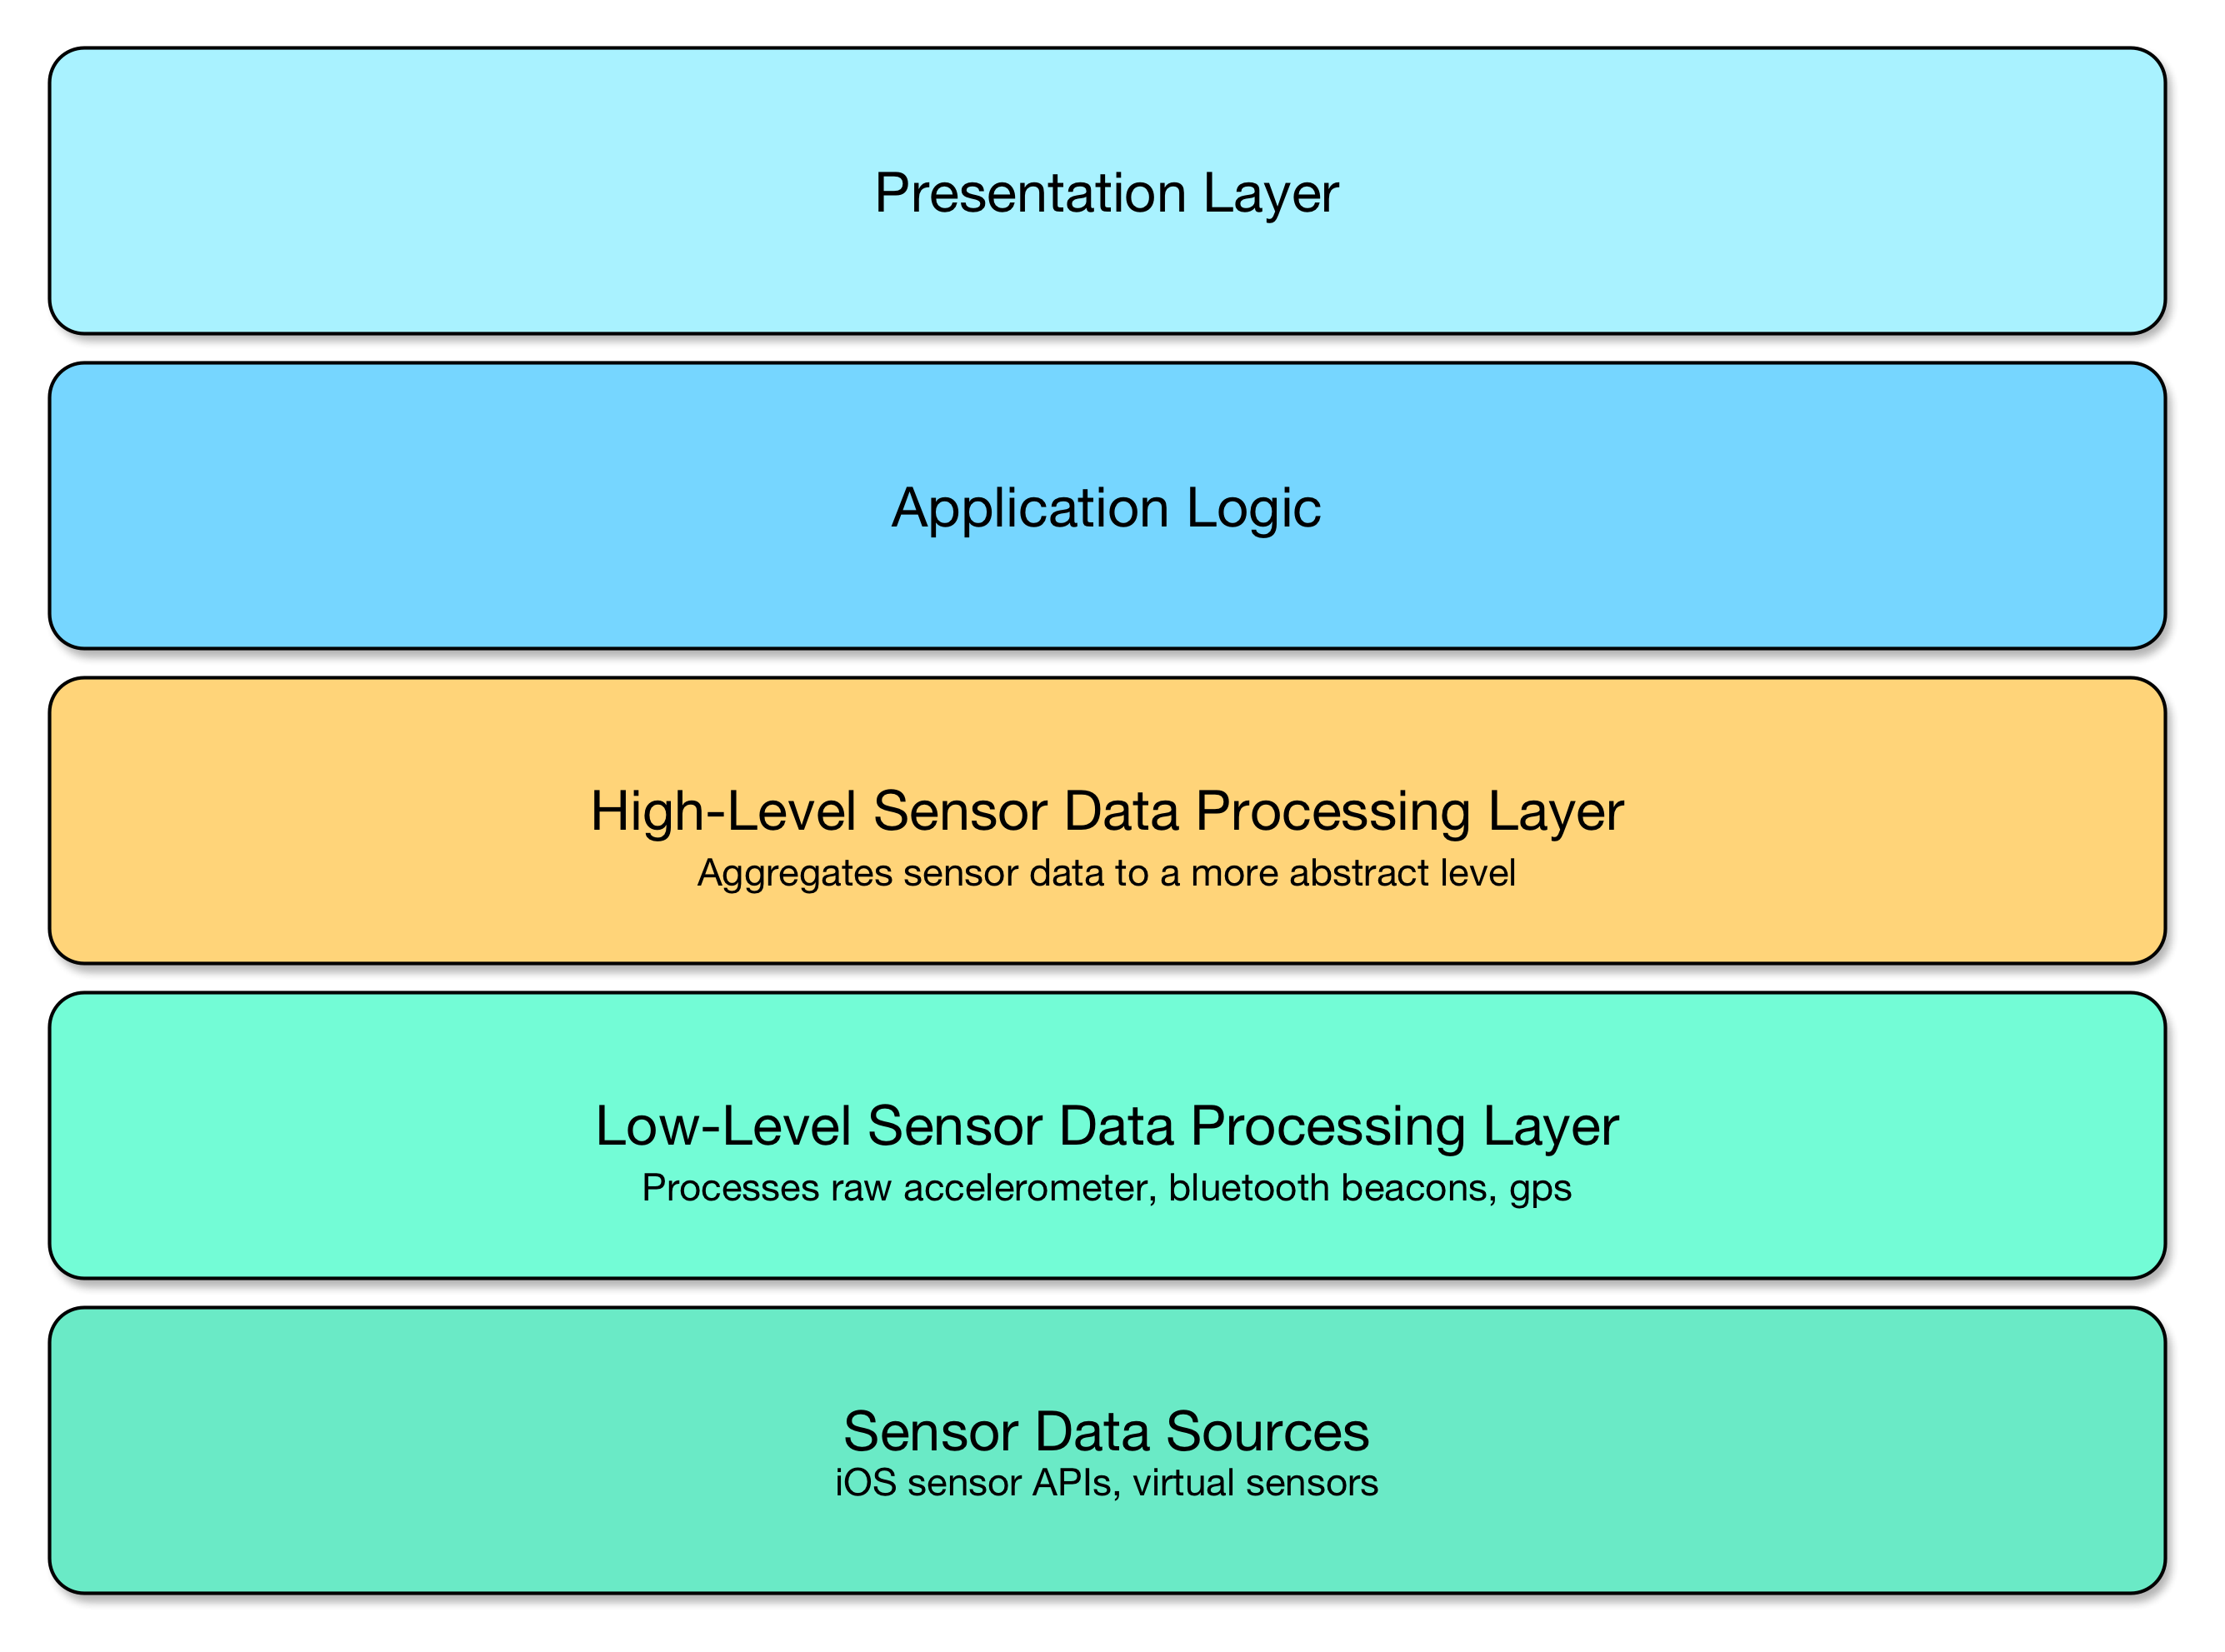
\includegraphics[width=0.7\textwidth]{layers-guide-app.png}
\caption{Layer model of the guide front-end}
\end{figure}

A fundamental requirement for the guide front-end, from a developer point of view, is the ability to record and replay recorded sensor readings of all accessed sensors and to automatically test single processing steps using recorded sensor data for comparing it with it's expected result.
To achieve this goal, virtual sensors are introduced at three different levels of abstraction inside the lower layers as depicted by the following figure.
 
 %TODO Beacons to HL, rest to App Logic
\begin{figure}[H]
\centering
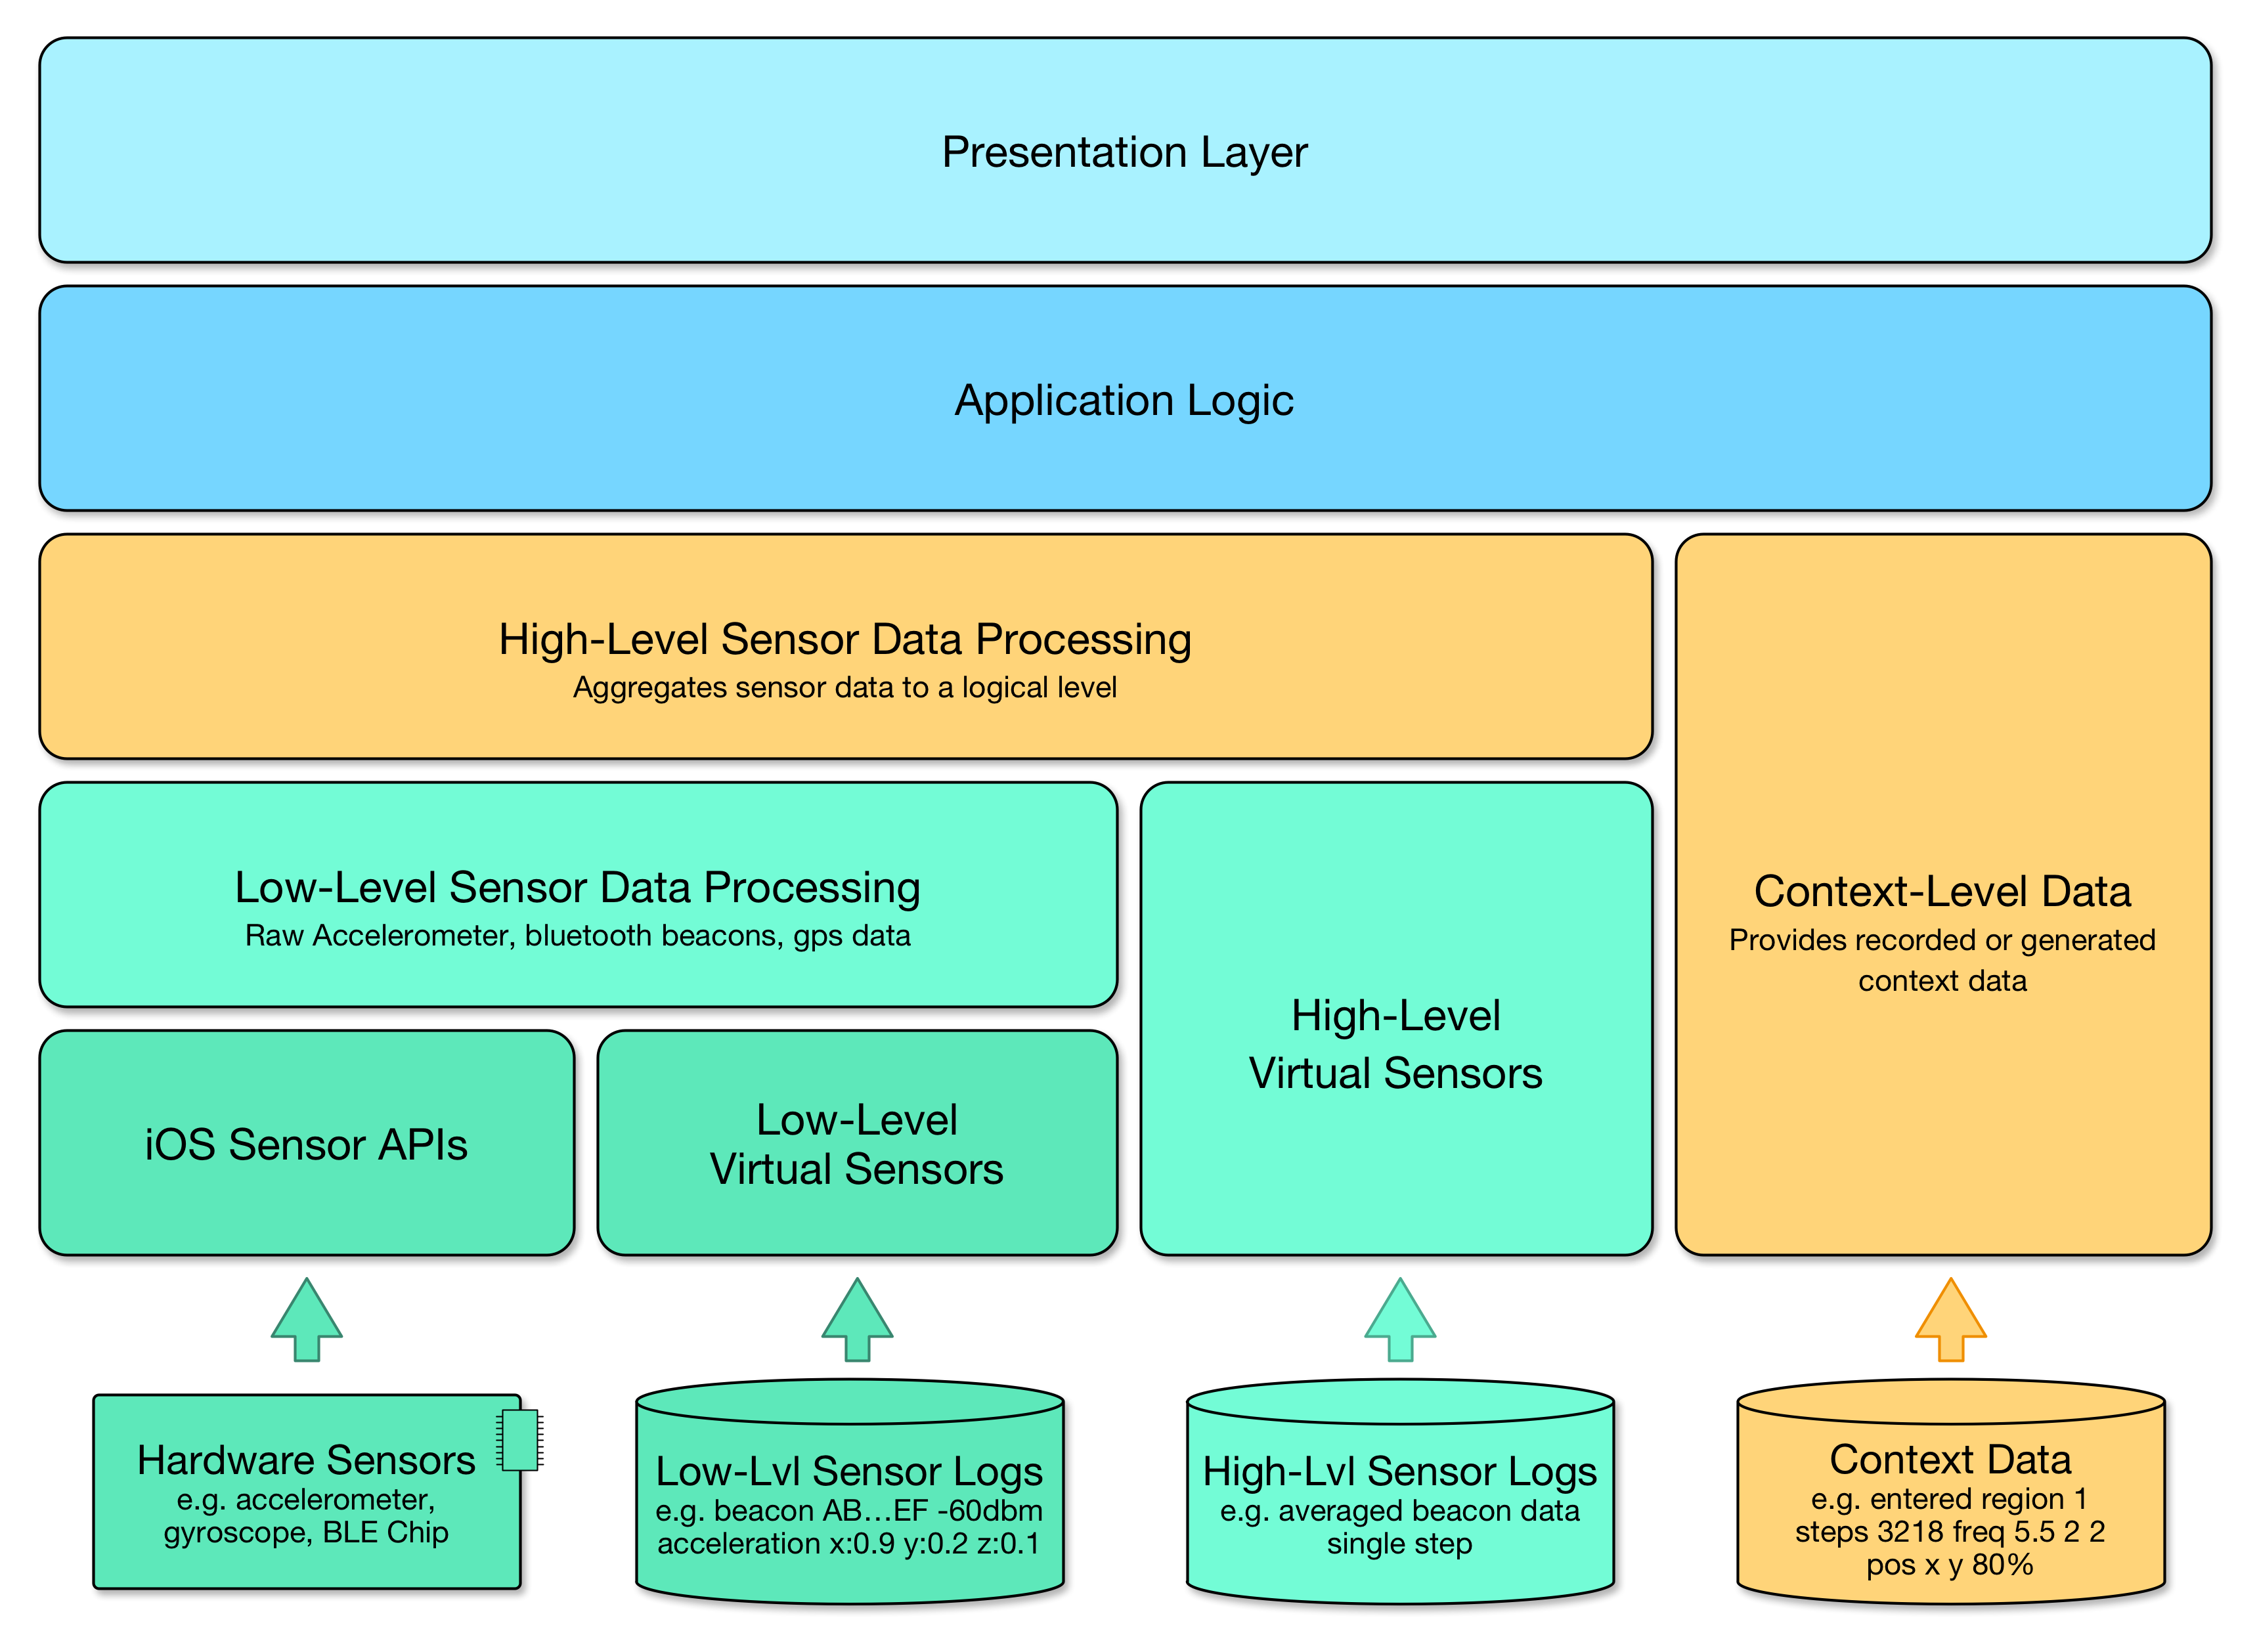
\includegraphics[width=0.9\textwidth]{layers-guide-refined-app.png}
\caption{Layer model with virtual sensors}
\end{figure} 

A virtual sensor delivers the same kind of data the processing algorithm of the corresponding layer would output, loading a previously recorded trace from the database. 
Also depicted are the external input data coming from the JSON site aggregate, containing the positions of all beacons with combined with their advertising data, the area geographic definitions and and the guide resources. The high-level sensor data processing layer uses the beacon related data for indoor positioning.

Figure~\ref{fig:dataflow} visualizes the different kind of data that is handled in every different layer, taking the accelerometer data processed by pedometer and statistics algorithms as an example. 

\begin{figure}[H]
\centering
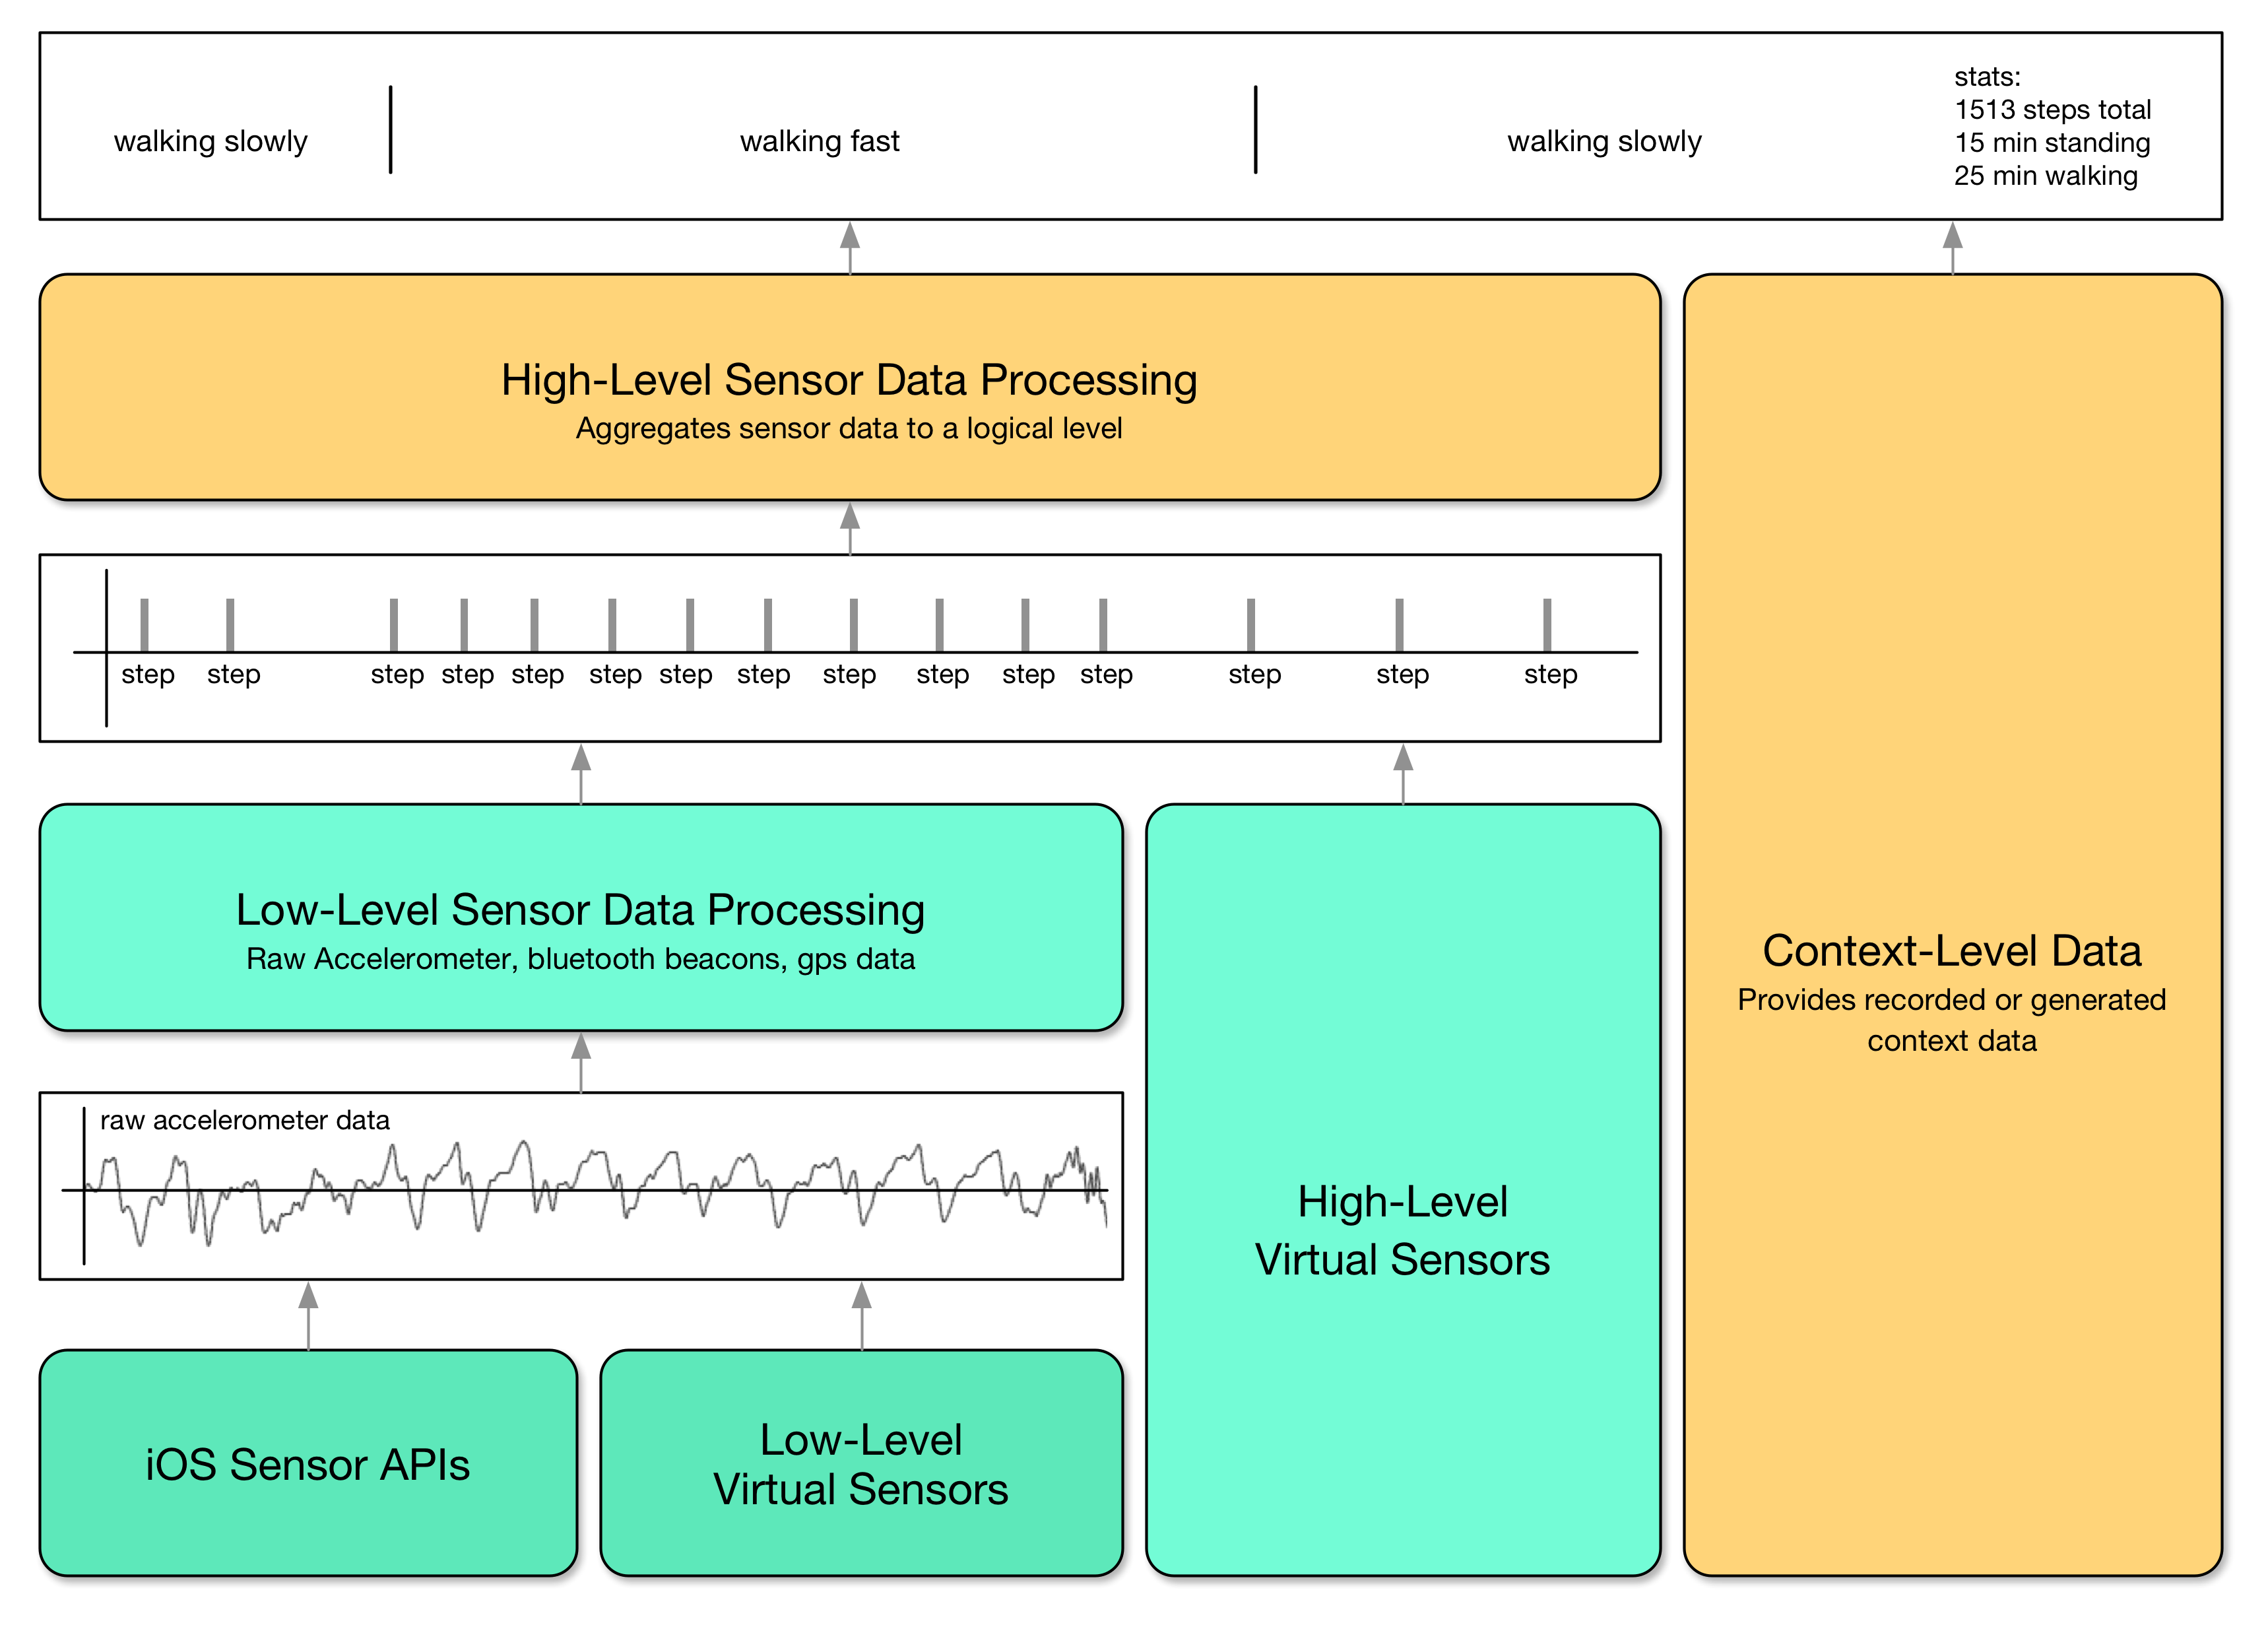
\includegraphics[width=0.9\textwidth]{layers-app-dataflow-accelerometer.png}
\caption{Data flow between the lower layers of the Sensorbase framework}
\label{fig:dataflow}
\end{figure}

The pedometer algorithm in the low-level sensor data processing layer receives raw accelerometer data as input. It analyzes the data, detects single steps and passes them to the upper layer, the high-level sensor data processing. Here the single steps are aggregated to periods of slow and fast walking and walking statistics are updated.\\
For most types of sensor data and information to be extracted, a processing approach using algorithms split in two layers can be found. For the rest the second layer could be omitted without affecting the other sensors. All the sensors implemented for this thesis use the two step processing approach.

The frequency of events passed to the next layer decreases from real-time (100 updates per second), demanding very fast algorithms, to some seconds or minutes. The following sequence diagram visualizes the decreasing frequency of updates from the lowest to the highest sensor related layer.

\begin{figure}[H]
\centering
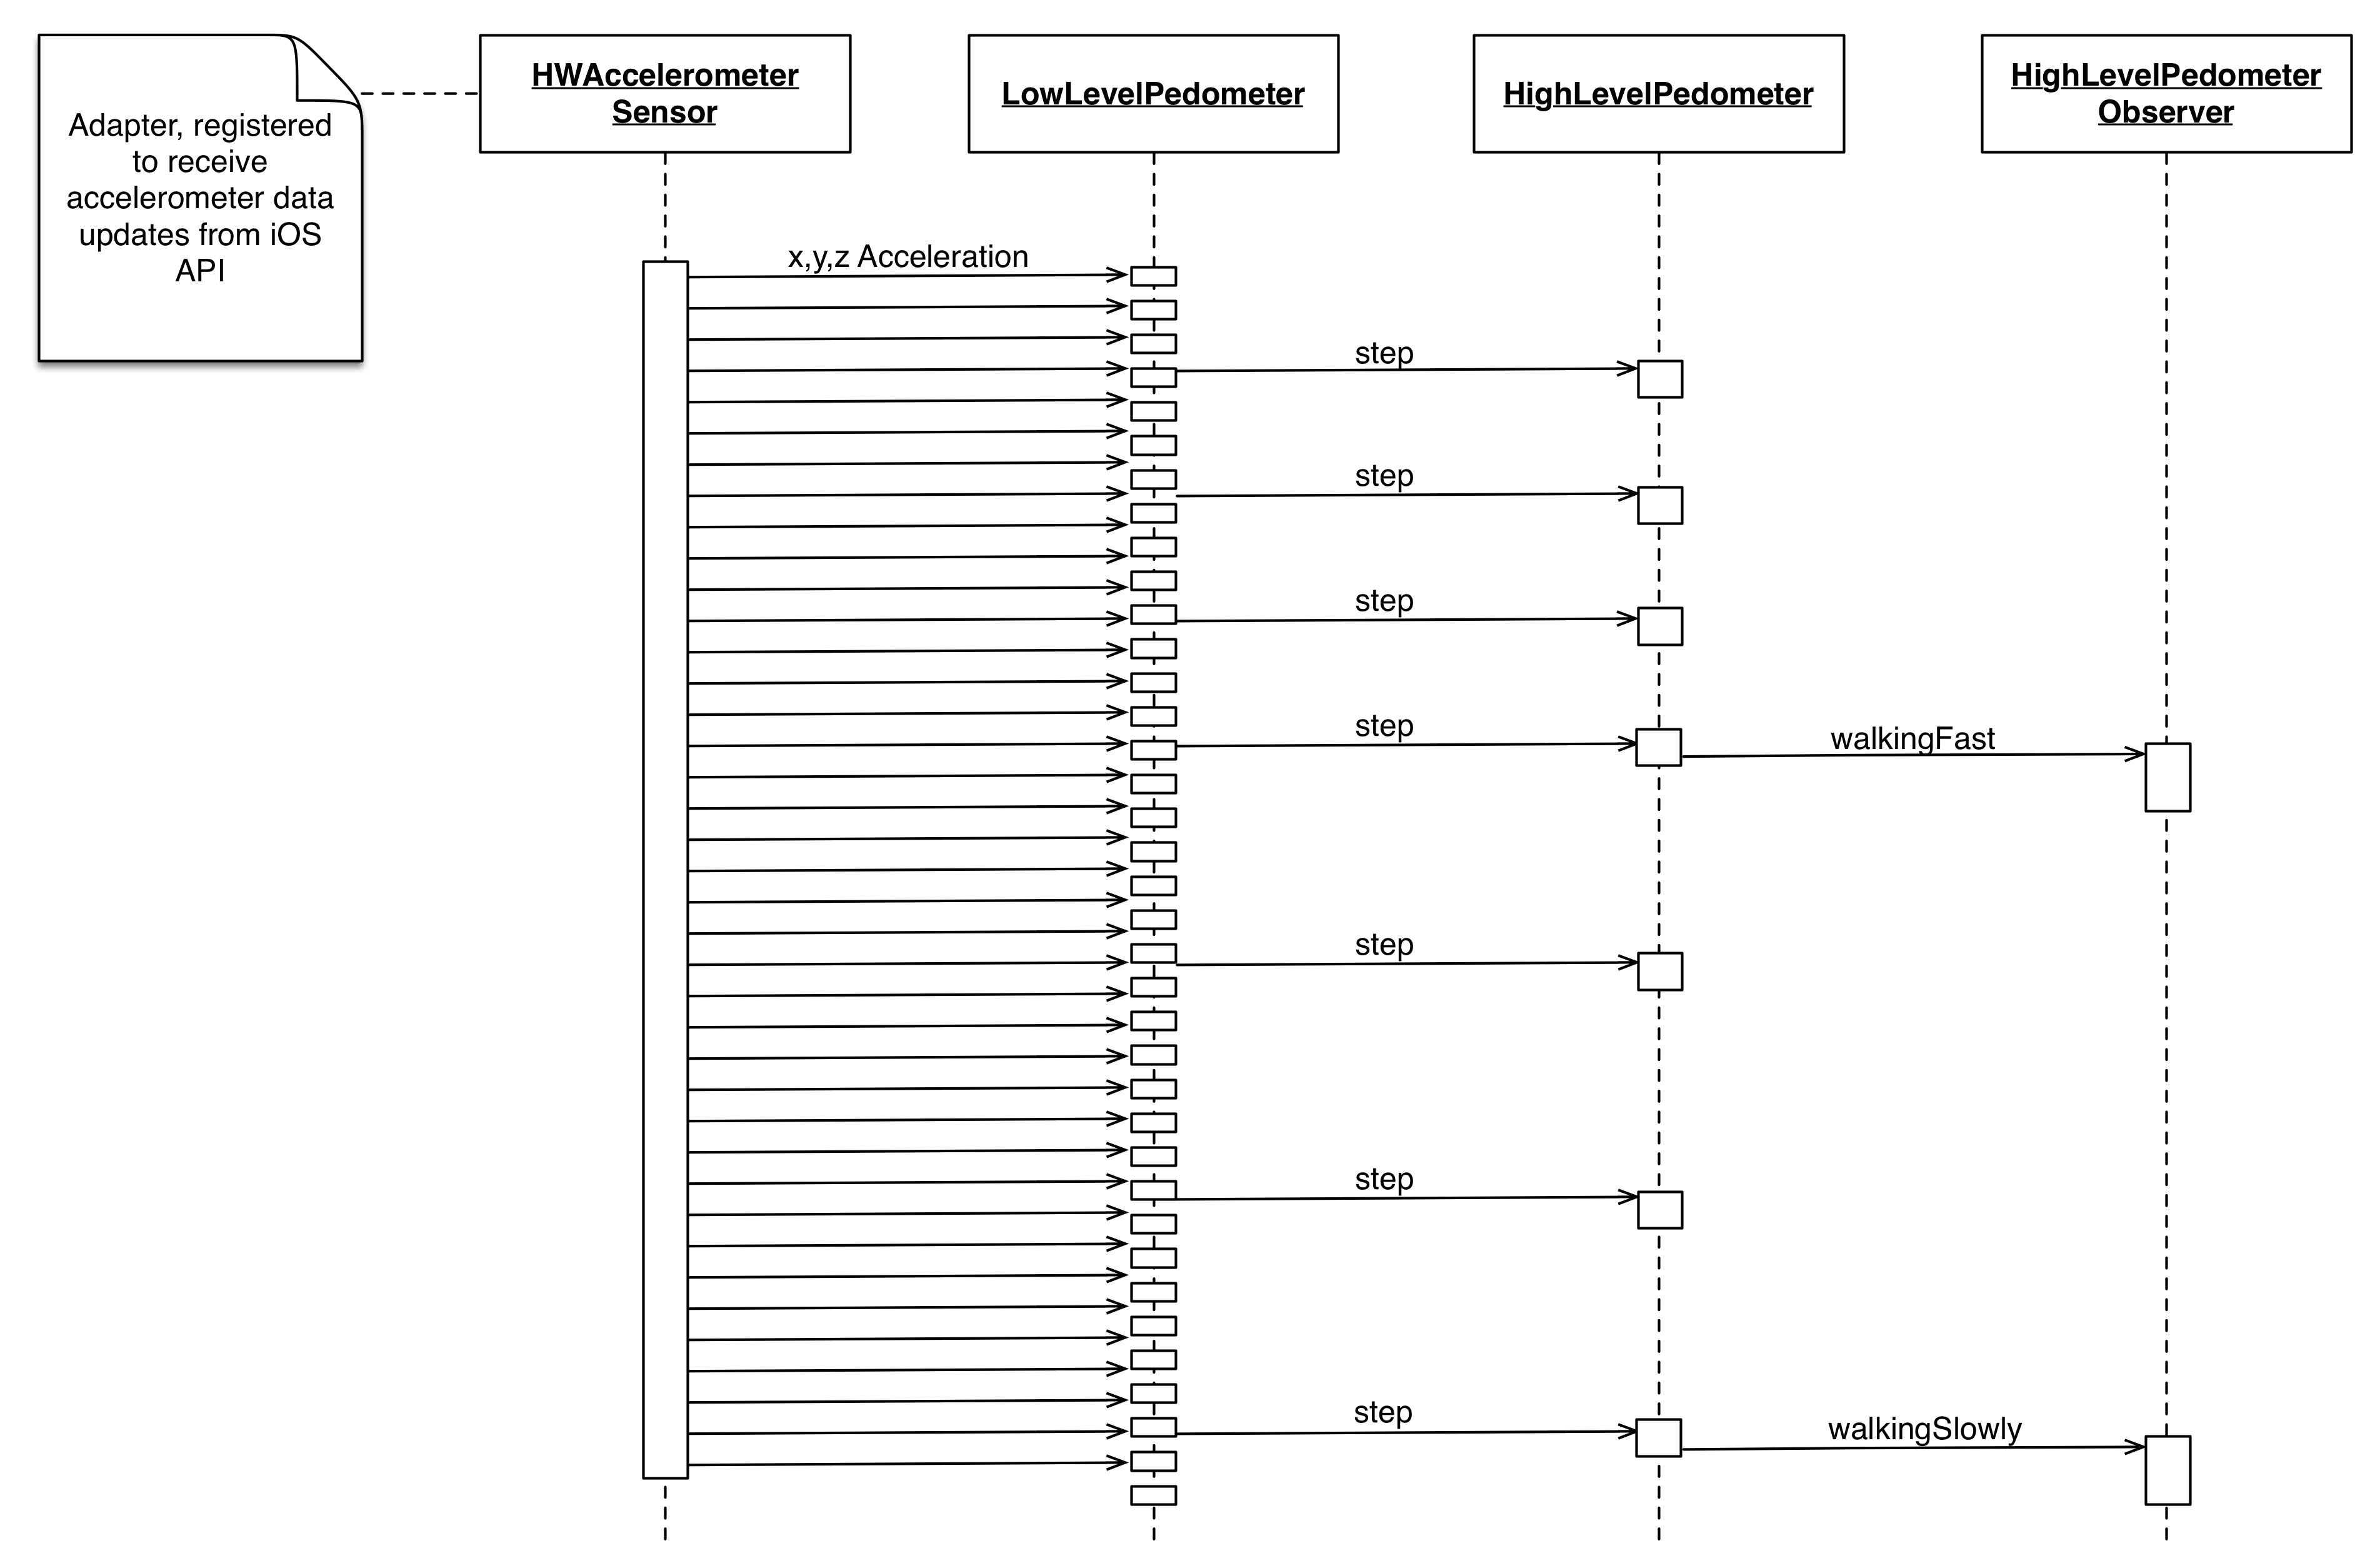
\includegraphics[width=1.0\textwidth]{sequence-diagram-sensorbase}
\caption{Sequence Diagram for the Sensor Layers}
\end{figure}

Beside enabling automated unit tests at different abstraction levels, this layered virtual sensor concept has various other benefits:

\begin{itemize}
\item During development, a simulation of walking through a park or museum is possible, for manually testing not only algorithms of the lower layers, but also elements of the uppermost layer like different screen transitions or other UI behavior.
\item For demonstrating the guide to customers or prospects, a walk through a park or museum can be simulated at the desk on a real device running the guide, beeing much more intuitive than showing only screen shots.
\item With an own class in the sensor data sources layer acting as an adapter to the iOS APIs it is easier to migrate the algorithms to a different mobile platform, by rewriting this adapter class for the target platforms sensor API and automatically translating the other sources that have no dependencies to the platform.
\end{itemize}

With the last point in mind, the value classes holding sensor data were only used in the lowest layer and converted to own iOS independent classes for further processing.



\begin{figure}[H]
\centering
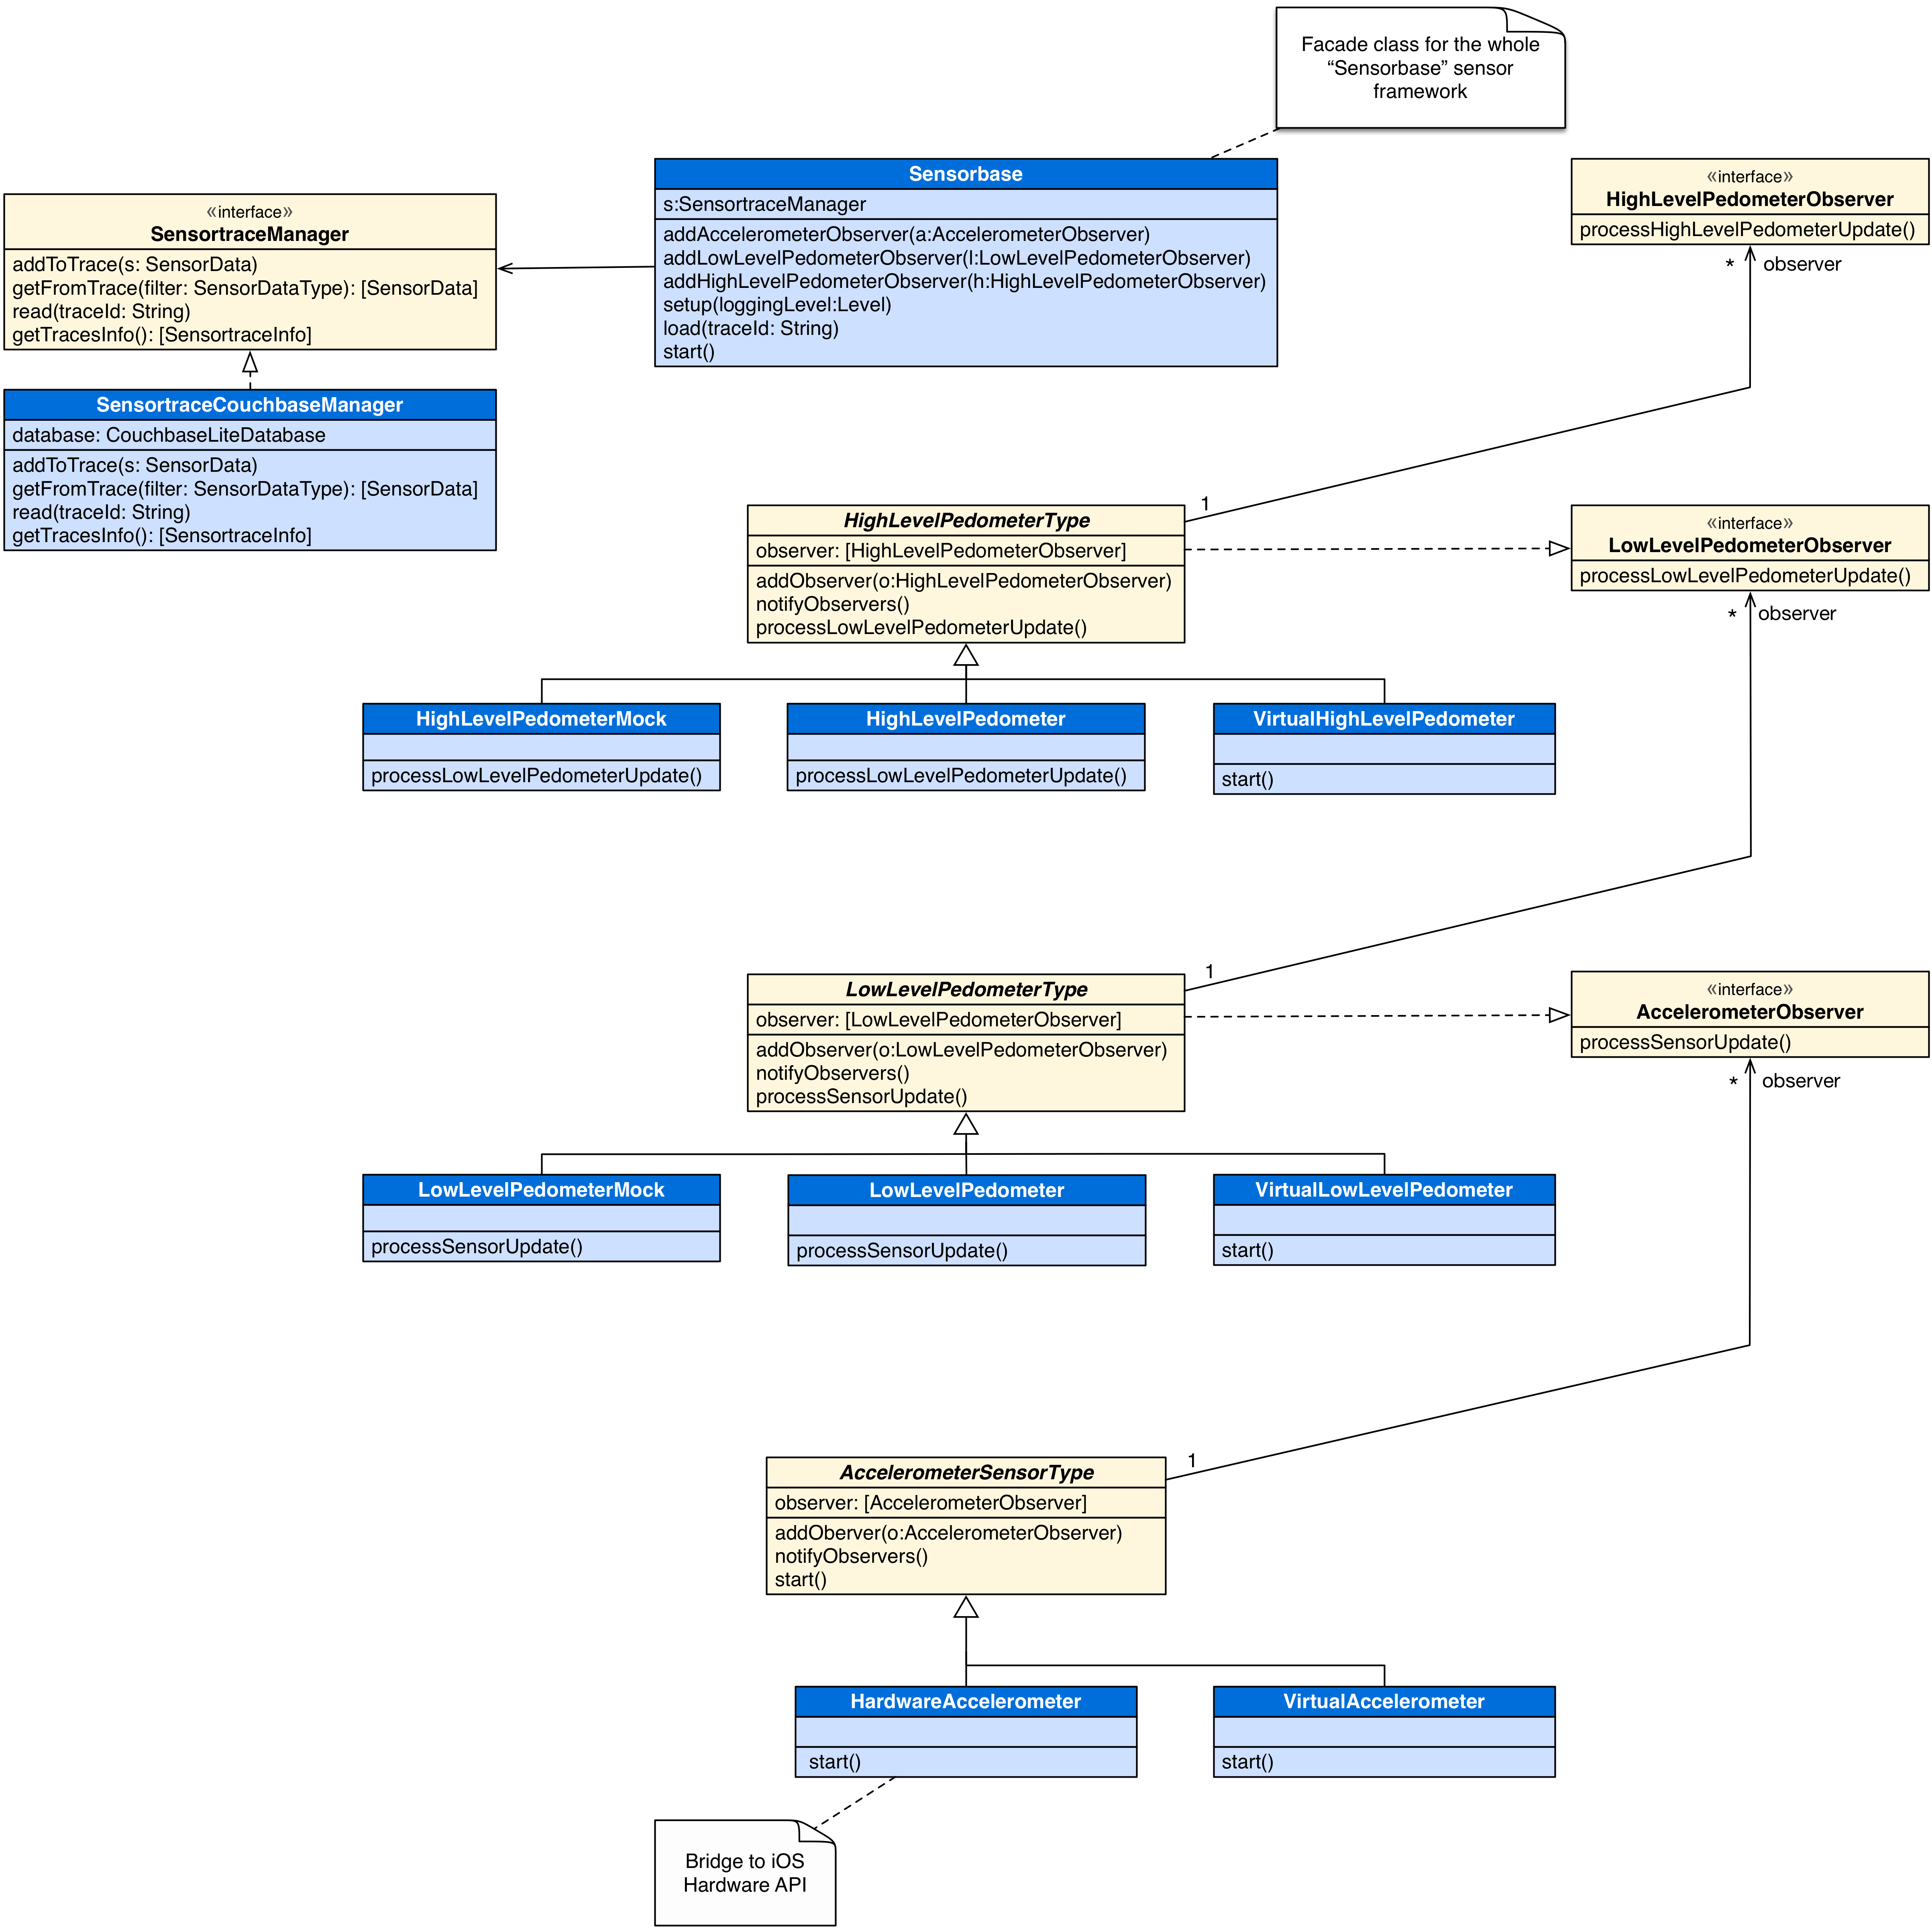
\includegraphics[width=1.0\textwidth]{class-diagram-guide-app.png}
\caption{Simplified Class Diagram for Sensor Data Processing}
\end{figure}

Mock: useful for Testing the underlying layer,
Adapter for iOS Sensor API,
The Sensorbase class is a singleton and acts as facade for the whole framework. It provides a single interface to the set of interfaces of the sensorbase subsystem. Knowing which subsystem class is responsible for which call, it delegates client requests to the appropriate subsystem object (cf. \cite{gof}).


\section{Sensors Layers}

Sensor data is saved to couchbase database.
Later access for replay (development), testing and presentations.
The backend can access this saved data for later analysis.

Sensorbase debug view.
\cite{GCD-Reference}

\subsection{Querying the Mobile NoSQL Database}
\label{sec:nosql-query}

When the key of the document to retrieve is known, the JSON document can be retrieved by simply using a getter function on the database object. All other queries are performed quite differently from standard databases. 

In the debug view, for example, a list of all recorded trace documents has to be displayed to allow the user selecting a trace for replaying it.
To perform this query in Couchbase Mobile and Swift, first a named view has to be created. A Couchbase view follows the map/reduce paradigm and thus a map and an optional reduce function have to be defined. 

In the current implementation of the Couchbase driver, the map function is defined using an Objective-C block that is automatically imported as Swift closure. That closure will be called internally on every document with the document itself and an emit function as parameters. The emit function can be called 0..* times for a single document with a key and value parameter. 

\begin{lstlisting}[basicstyle=\footnotesize,caption=The map function of the traces view]
// Setup the views
let tracesView = self.database.viewNamed(self.tracesViewName)
tracesView.setMapBlock({ (doc, emit) in
  if let timestamp = doc["timestamp"] as? String {
    if let site = doc["site"] as? String {
      if let data = doc["data"] as? [AnyObject] {
        emit([site, timestamp, data.count], doc["_id"])
      }
    }
  }
}, version: "3")
\end{lstlisting}

Being a very young language, new versions of Swift were released during this work. So one improvement of Swift 1.2, released on 9th February 2015 \cite{swift-1-2}, was allowing multiple optional value bindings inside a single if statement, avoiding deeper nesting levels seen above. 

\begin{lstlisting}[basicstyle=\footnotesize,caption=The map function avoiding nesting with Swift 1.2,language=Swift]
// Setup the views, Swift v1.2
let tracesView = self.database.viewNamed(self.tracesViewName)
tracesView.setMapBlock({ (doc, emit) in
  if let timestamp = doc["timestamp"] as? String, 
    site = doc["site"] as? String, 
    data = doc["data"] as? [AnyObject] {
      emit([site, timestamp, data.count], doc["_id"])
  }
}, version: "3")
\end{lstlisting}

The key can be a single value or a list of values, as seen here, useful for later querying using start and end barriers on single elements of the key list, as shown later. The emitted key for the sites view is built with the site's id, the timestamp of the trace and the number of measurements inside the document. 

The view can be thought of as an index in a conventional database - not a query. Couchbase uses the view definition with it's map and reduce function to create it's internal indices. Once created, the view can then be used to instantiate a query, configure it and retrieve the desired data.

For example, to create a query returning only sensor traces for the site "Site-CXN01" that were created after 1st January 2015 (1420070400 as Unix timestamp) using the previously defined sites view, the startKey and endKey properties can be defined the following way.

\begin{lstlisting}[basicstyle=\footnotesize,caption=Setting up the NoSQL query,language=Swift,label=lst:nosql-query]
let tracesView = database.viewNamed(tracesViewName)
let query = tracesView.createQuery()
query.startKey = ["Site-CXN01",1420070400]
query.endKey   = ["Site-CXN01",[:]]
\end{lstlisting}       

The empty dictionary used as second element of the end key is Couchbase value sorted always at the end and the preferred way to define an upper bound greater than all existing elements.

A single view can be queried by defining a coherent range of the ordered keys. While it is possible to limit the timestamp value inside a single site with this view, to select a timestamp range with arbitrary sites a new view has to be defined, emitting the timestamp as first key element.

The reason is Couchbase organizes it's data holding a sorted index of the emitted keys. For multi-element keys, they are sorted primarily by the first key element, then by the second and so on.

\begin{figure}[H]
\centering
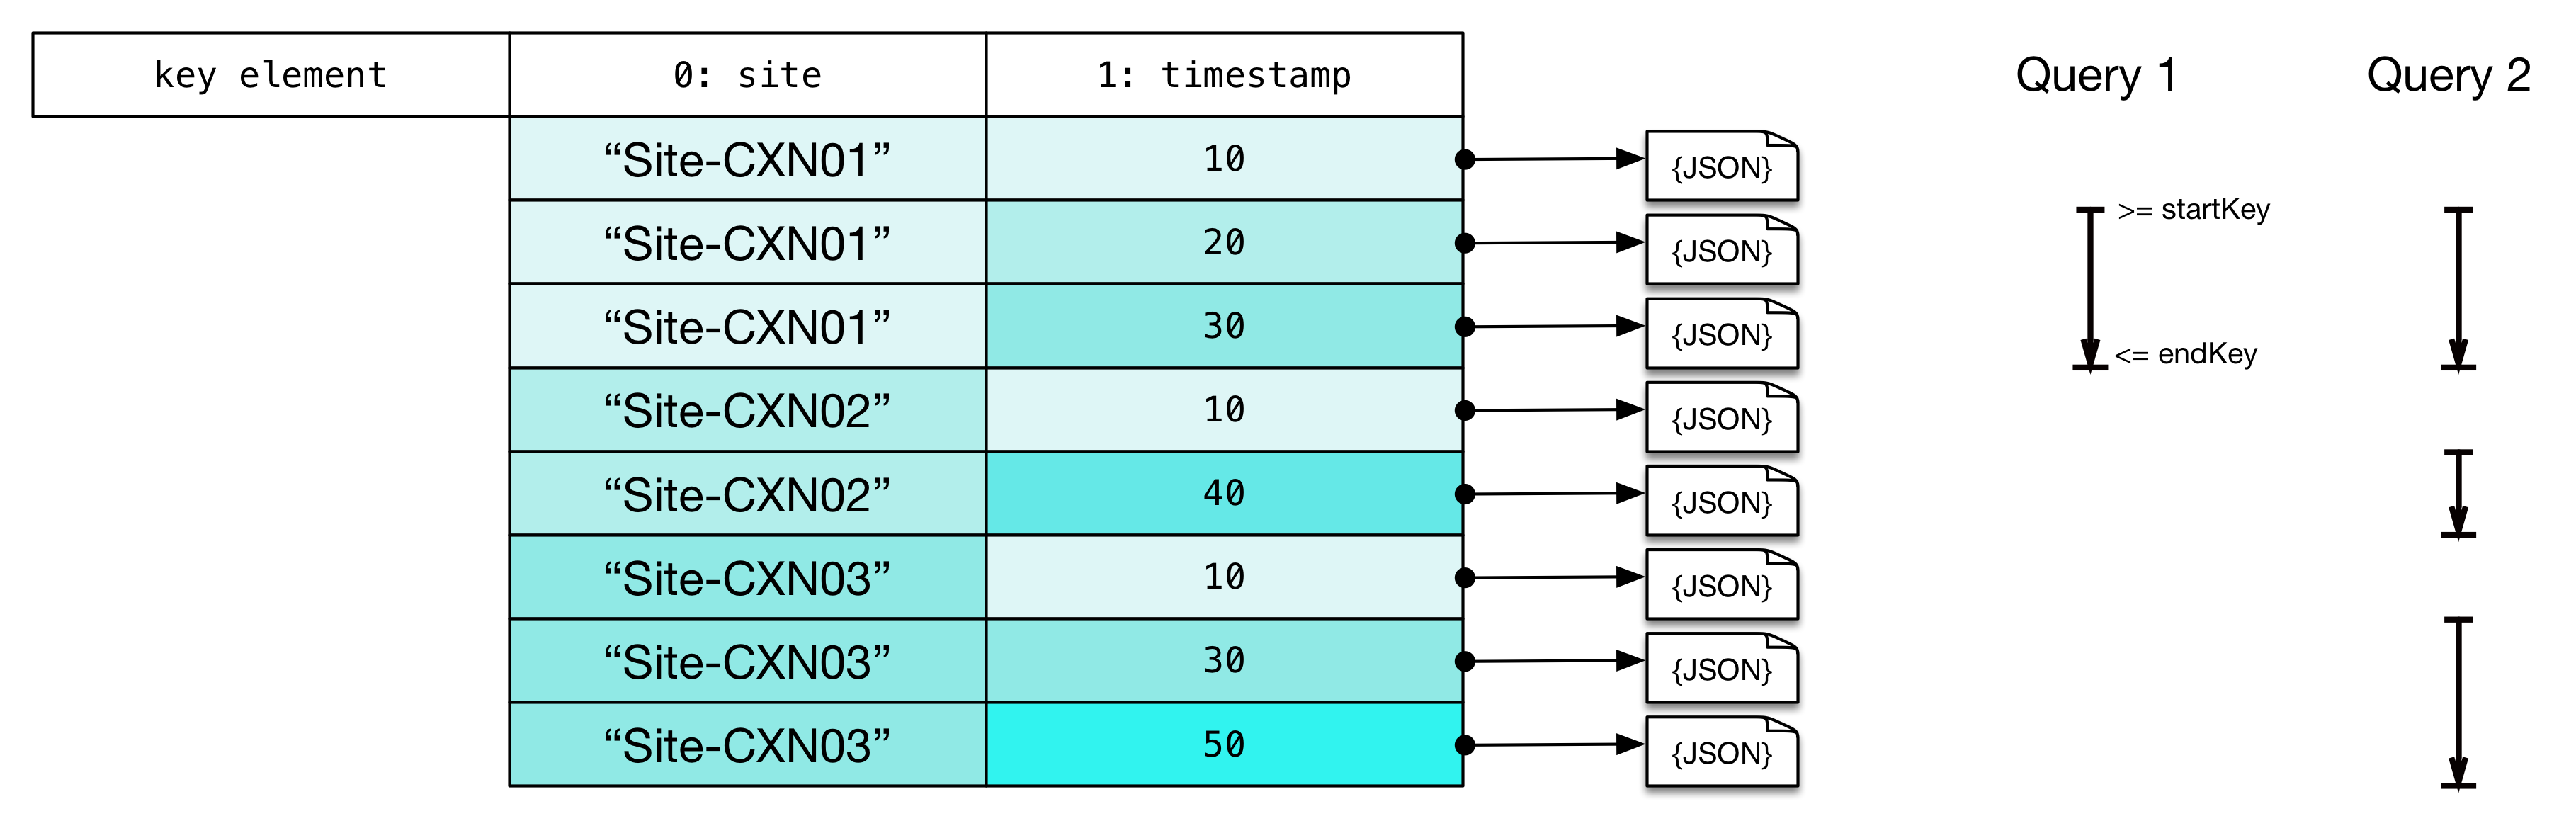
\includegraphics[width=0.9\textwidth]{couchbase-query}
\caption{Couchbase limits for querying views}
\label{fig:couchbase-query}
\end{figure}

Figure~\ref{fig:couchbase-query} visualized the index with a simplified key consisting of two elements: the site id and the timestamp. The first query is equivalent to the on of listing~\ref{lst:nosql-query}. Selecting only timestamps >= 20 for arbitrary sites would result in the scattered ranges pictured by query two. Therefore query 2 cannot be expressed by defining a start and end key on this view.

That's the price to pay for the focus on high performance and the automatic scaling capabilities of Couchbase and similar NoSQL databases. Although, compared with the benefits, this extra work seems reasonable.

Finally, running the query is similar to known relational database drivers. 

\begin{lstlisting}[basicstyle=\footnotesize,caption=Performing the NoSQL query,language=Swift]
var error: NSError?
let result = query.run(&error)
var found = false
while let row = result?.nextRow() {
   // do something with the row
}
\end{lstlisting}


\section{Application Logic}

For this work, the application logic on top of the sensor layers focuses on computing the area that contains the position obtained by the lower layer. This is done using computational geometry algorithms described in  %TODO



For the final product, the guide has to keep track of the audio files already played and decide if it is appropriate to play the lower levels of detail based on the current walking speed and the size of the area.

If so and some other rules apply, the content is presented to the user in the appropriate way.

If not walking fast load and play current content.

If display is on show actions that user has to opt in, if display is off play automatically. 

\section{Presentation Layer}

%TODO2 Study with parallax

The full design of the front-end GUI is out of scope of this thesis, which limits the presentation layer to the debugging dashboard.
This view shows processed and unprocessed sensor data of different layers, and contains controls for loading and saving sensor traces. Even after adding the end-user GUI, this debugging dashboard will remain in the application for development and testing.

A mockup of the debugging dashboard was designed using the tool "Balsamiq Mockups" \cite{balsamiq}.

\begin{figure}[H]
\centering
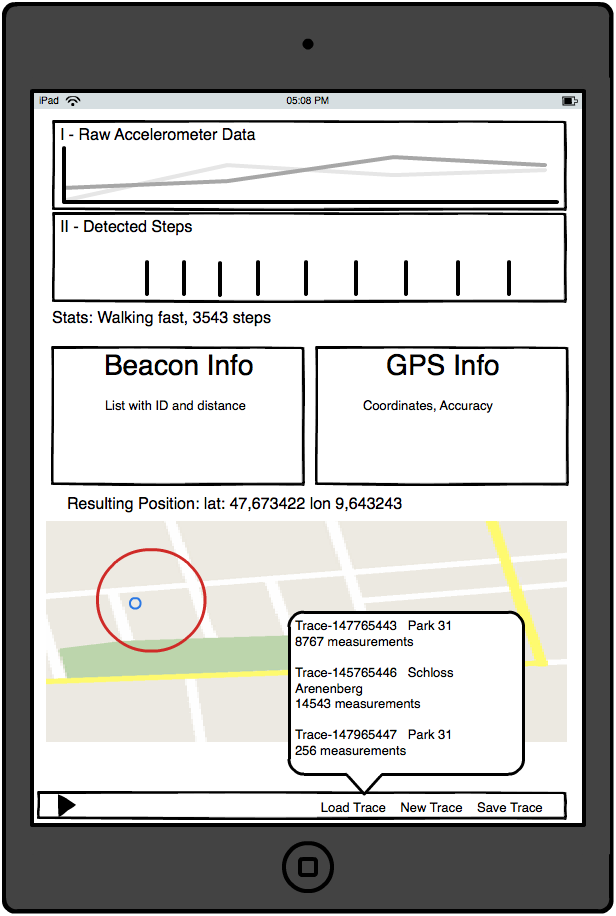
\includegraphics[height=0.4\textheight]{mockup-guide-debug}
\caption{A mockup of the debug dashboard}
\label{fig:couchbase-query}
\end{figure}

On the top, the raw accelerometer data is depicted in a chart with the acceleration force on it's vertical axis and the time on it's horizontal axis. Below, a graph shows vertical peaks every time a step is detected. The statistics of the third layer are visible as text showing the walking speed and the cumulated steps.
The beacon info section consists of a list of all currently sensed beacons with their properties. Beside, a GPS section shows all GPS related data. The resulting position is additionally shown on a map using a blue circle, with an optional red circle for the pure GPS position and accuracy, depicted as radius of the circle. On the bottom of the screen, a toolbar contains all controls needed for managing the sensor traces. The load trace action has to show a list of all traces (cf. section~\ref{sec:nosql-query}) and loads the selected trace.

\begin{figure}[H]
\centering
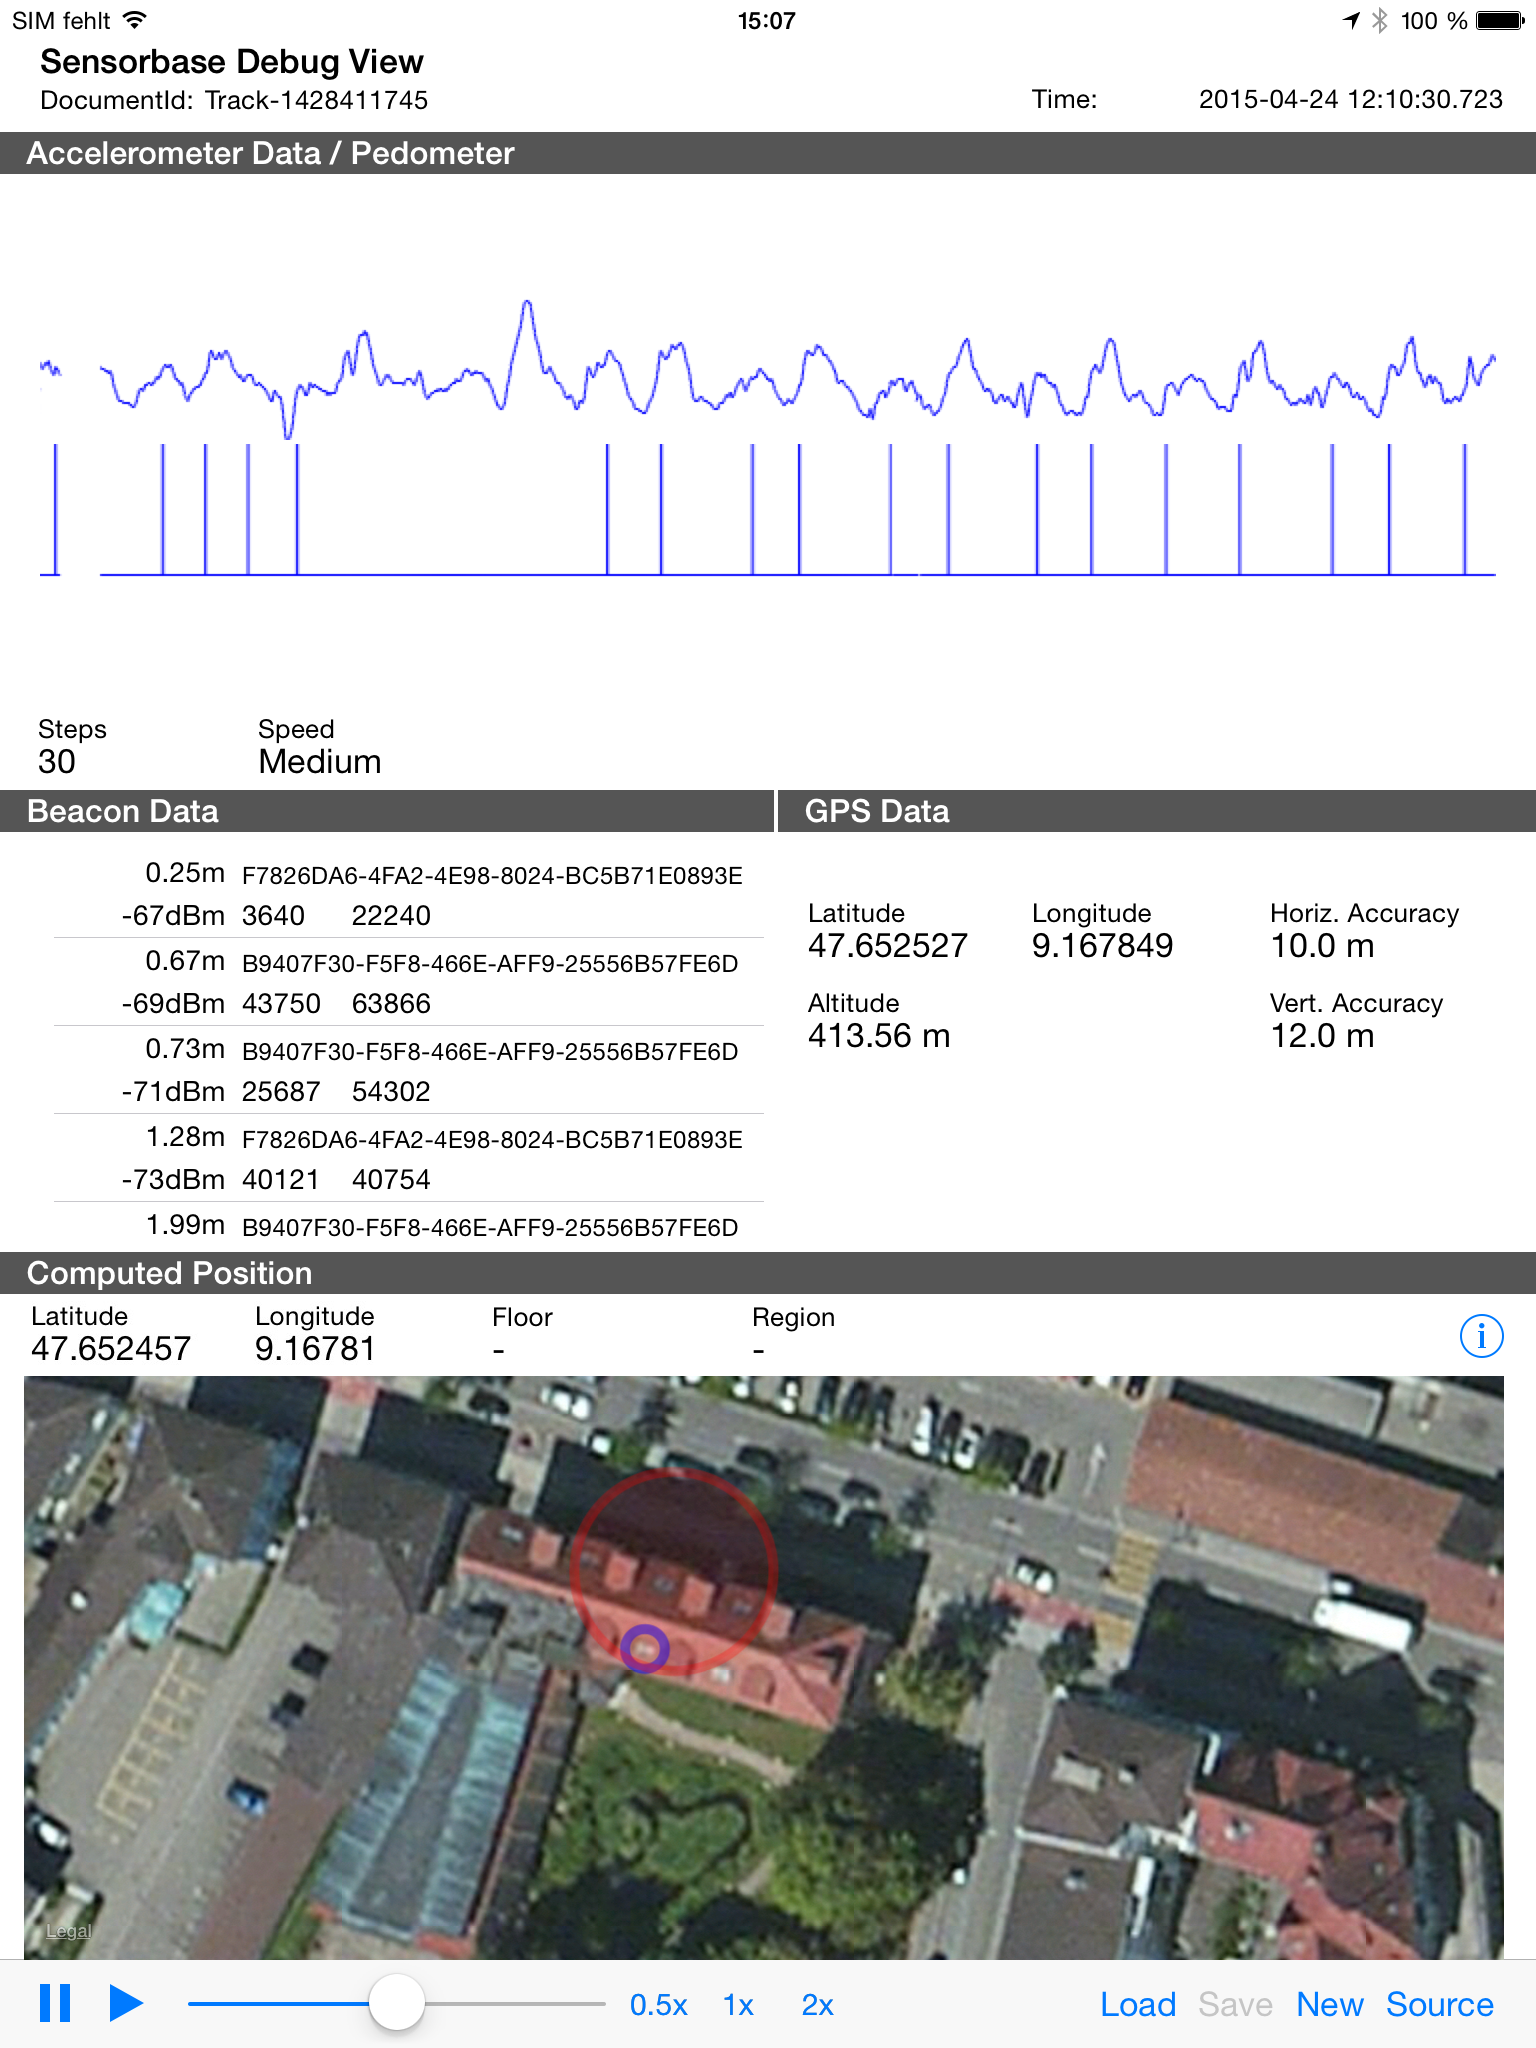
\includegraphics[height=0.4\textheight]{screen-debug-view}
\caption{Screenshot of the debug dashboard running on an iPad}
\label{fig:couchbase-query}
\end{figure}

\section{Summary}

We now have a mobile system capable of processing sensor readings in several layers and recording and replaying them at a desired level of detail. 
The system loads sites defined as JSON document and uses the beacons definitions to locate itself when GPS signal is missing or not accurate. Based on the current position and the loaded area definitions, the current area is computed and the content loaded.

The next chapter handles the design and implementation of the second part of the framework: The back end serving as site modeling and analytics tool.